% Provenance (never printed): old premiere S material on the lithosphere and the
% asthenosphere (chemical and mechanical layers, the low-velocity zone, the
% geotherm, isostasy); see sources/book2/PROVENANCE.md. S speeds from
% figdata/grade-11/prem_profiles.py (part upper), the geotherm and the solidus
% from geotherm_solidus.py, the elevations from hypsometry.py (ETOPO1).
% Glacial rebound belongs to g12; lithostatic pressure (term) to g12.
\chapter{岩石圈与软流圈}\label{ch:g11:lithosphere-asthenosphere}

冰山有九成的体积位于水下：冰之所以能够漂浮，是因为它
密度略小于海水，它沉入水中，直到排开的水重恰好等于整座冰山的重量。
山脉的情形与此大致相同。在最高的山脉之下，地壳
厚度接近通常的两倍，
多出的地壳大部分隐藏在下方，如同水线以下的冰。
但冰山漂浮在液体中，而山脉之下的地幔是固态岩石。
本章说明，固体如何能像一种流体那样表现，使地球的外壳漂浮其上，
以及这一外壳究竟是什么。
% ledger: usgs:ice-density, karplus:tibet-moho, cm95:crust

\begin{recall}
地球分为地壳、地幔和地核（第 1 册，六年级）。\omterm{def:g11:seismic-structure:moho}{莫霍面}位于
地壳底部，平均而言在大陆之下深约 \qty{41}{km}，
在洋底之下则仅几千米；
地震波速度和密度在各深度的数值都可由地球参考模型得知
（见\cref{ch:g11:seismic-structure}）。岩石随深度增温，
近地表时每千米约升高 25 至 \qty{30}{\celsius}（第 1 册，六年级）。
漂浮在液体中的物体，排开的液体重量等于自身重量，
而柱状物质底部的压强，等于柱体的重量除以其面积
（物理课本）。
\end{recall}
% ledger: cm95:crust, usgs:crust-thickness, usgs:gradient-29 (Book 1 rows)

\begin{omfigure}
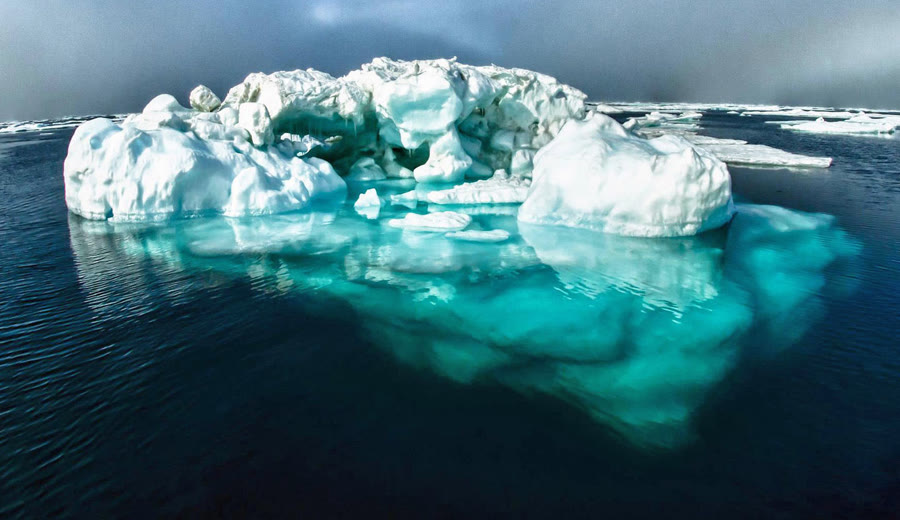
\includegraphics[width=0.66\linewidth]{images/book2/g11-noaa-iceberg.jpg}

{\small 从水面上方看到的冰山：水面之下的冰，
透过清澈的海水可见，远比露出空中的部分大得多。
照片：NOAA，公有领域。}
\end{omfigure}
% ledger: photo:g11-iceberg

\section{地球分层的两种方式}

地壳、地幔和地核是由不同
\emph{材料}构成的层：地壳由富含硅、铝和
氧的岩石构成，地幔由密度更大的岩石构成，地核由金属构成。
但地球的外部还可以按岩石在受力时的
\emph{行为}方式来划分，这些力可以持续很长时间。

\begin{definition}[岩石圈；软流圈]\label{def:g11:lithosphere-asthenosphere:lithosphere}
称\emph{岩石圈}\index{岩石圈}为地球的刚性外壳，
即地壳与地幔最上部、温度最低的部分，
共同破裂成构造板块，且不发生流动。
\emph{软流圈}\index{软流圈}是位于岩石圈之下的地幔层，
温度更高、强度更弱，在漫长的时间尺度上缓慢流动，
如同极为黏稠的糊状物。
\end{definition}

二者的界面位于海洋和大多数大陆之下约 70 至 \qty{100}{km} 深处，
而在大陆最古老的部分之下更深；
以美国为例，\omterm{def:g11:lithosphere-asthenosphere:lithosphere}{岩石圈}厚度从西部的
约 \qty{40}{km} 增至大陆中部 \qty{200}{km} 以上。
\omterm{def:g11:lithosphere-asthenosphere:lithosphere}{岩石圈}的底面并非\omterm{def:g11:seismic-structure:moho}{莫霍面}，\omterm{def:g11:lithosphere-asthenosphere:lithosphere}{岩石圈}的大部分
是地幔岩石。
% ledger: rs09:lab, fischer:lab, porter:lab, usgs:lithosphere-80km (Book 1 row)

\begin{omfigure}
\begin{tikzpicture}[x=1cm, y=-0.0125cm, font=\footnotesize]
% depths to scale: crust 41 km (cm95:crust), lithosphere 100 km (rs09:lab), 0-400 km
  \shade[top color=omLithPeridotite!70, bottom color=omLithPeridotite!25] (5,100) rectangle (8,400);
  \fill[omLithGranite!55] (0,0) rectangle (3,41);
  \fill[omLithPeridotite!55] (0,41) rectangle (3,400);
  \fill[black!25] (5,0) rectangle (8,100);
  \draw (0,0) rectangle (3,400);
  \draw (5,0) -- (5,400) (8,0) -- (8,400) (5,0) -- (8,0);
  \draw[line width=0.8pt] (0,41) -- (3,41);
  \draw[line width=0.8pt, densely dashed] (5,100) -- (8,100);
  \draw[densely dotted, black!60] (3,41) -- (5,41);
  \node at (1.5,20) {地壳};
  \node[align=center] at (1.5,220) {地幔};
  \node[align=center] at (6.5,50) {岩石圈 \\刚性};
  \node[align=center] at (6.5,180) {软流圈 \\较弱，缓慢流动};
  \node[align=center, text=black!70] at (6.5,340) {深部地幔};
  \node[anchor=south, font=\small] at (1.5,0) {按材料};
  \node[anchor=south, font=\small] at (6.5,0) {按行为};
  \foreach \d in {0,100,200,300,400} {\draw (-0.1,\d) -- (0,\d); \node[anchor=east] at (-0.1,\d) {\d};}
  \node[anchor=east, rotate=90, anchor=south] at (-0.9,200) {深度（\unit{km}）};
  \node[anchor=south, font=\scriptsize, align=center] at (4,41) {莫霍面 \\（\qty{41}{km}）};
  \node[anchor=west, align=left] at (8.15,100) {岩石圈底部 \\（约 \qty{100}{km}）};
\end{tikzpicture}

{\small 大陆之下地球的上部 \qty{400}{km}，按比例绘制。
左图：按材料划分的各层。右图：按行为划分的各层。刚性
\omterm{def:g11:lithosphere-asthenosphere:lithosphere}{岩石圈}包含整个地壳和地幔顶部；
\omterm{def:g11:lithosphere-asthenosphere:lithosphere}{软流圈}没有明确的下界。}
\end{omfigure}

\section{低速带}

地震波揭示了\omterm{def:g11:lithosphere-asthenosphere:lithosphere}{软流圈}。在地球内部几乎各处，地震波
速度随深度增大，因为岩石受到的挤压越来越强。在
\omterm{def:g11:lithosphere-asthenosphere:lithosphere}{岩石圈}之下，情况则恰好相反。

\begin{definition}[低速带]\label{def:g11:lithosphere-asthenosphere:lvz}
称\emph{低速带}\index{低速带}为上地幔中的一层，
位于\omterm{def:g11:lithosphere-asthenosphere:lithosphere}{岩石圈}之下，地震波在其中的传播速度比
上方和下方的岩石中都更慢。
\end{definition}

在\omterm{def:g11:seismic-structure:reference-model}{参考地球模型}中，\omterm{def:g11:seismic-structure:body-waves}{S 波}速度从\omterm{def:g11:seismic-structure:moho}{莫霍面}向下缓慢降低，
直到 \qty{220}{km} 深处，随后陡然回升。世界各地的地震研究都发现
在 70 至 \qty{100}{km} 之间某处有明显的速度骤降：
\omterm{def:g11:lithosphere-asthenosphere:lithosphere}{软流圈}的顶部。该处岩石温度足够高，已接近熔化，
可能含有极少量熔体；其含水量也可能高于上方的岩石。
接近熔化的岩石强度很低：它使地震波减慢，并且能够流动。
% ledger: data:prem, rs09:lab, fischer:lab, porter:lab

\begin{omfigure}
\begin{tikzpicture}
\begin{axis}[omrecord, omdepth, width=0.6\linewidth, height=6.0cm, xmin=3.0, xmax=5.0, ymin=0, ymax=400,
  xlabel={S 波速度 (\unit{km/s})}, ylabel={深度 (\unit{km})}, xtick={3.0,3.5,...,5.0},
  xticklabel style={/pgf/number format/fixed, /pgf/number format/precision=1},
  tick label style={font=\small}, label style={font=\small}]
% computed in figdata/grade-11/prem_profiles.py (part upper); ledger: data:prem
\fill[black!10] (axis cs:3.0,80) rectangle (axis cs:5.0,220);
\addplot[omProp, line width=0.9pt] table[x=vs, y=depth] {figdata/out/grade-11-prem_profiles-upper.dat};
\node[font=\scriptsize, anchor=west, align=left] at (axis cs:3.1,150) {低速 \\带};
\node[font=\scriptsize, anchor=west] at (axis cs:3.95,12) {地壳};
\end{axis}
\end{tikzpicture}

{\small \omterm{def:g11:seismic-structure:reference-model}{参考地球模型}上部 \qty{400}{km} 内的 \omterm{def:g11:seismic-structure:body-waves}{S 波}速度。
地壳之下，波速随深度缓慢减小，直至
\qty{220}{km} 深处（自 \qty{80}{km} 起着色），随后
以突变阶跃的方式再次增大。}
\end{omfigure}

\section{地温线}

\begin{definition}[地温线；地温梯度]\label{def:g11:lithosphere-asthenosphere:geotherm}
某地下方温度随深度变化的曲线称为\emph{地温线}\index{地温线}。
\emph{地温梯度}\index{地温梯度}是
单位深度上温度的升高量，单位为摄氏度每千米。
\end{definition}

钻孔仅能在最浅的几千米内测量\omterm{def:g11:lithosphere-asthenosphere:geotherm}{地温线}，该处
温度每千米升高 25 至 \qty{30}{\celsius}（第 1 册，
六年级）。更深处的\omterm{def:g11:lithosphere-asthenosphere:geotherm}{地温线}，由经地表流出的热量
与岩石性质计算得出；这些热量的来源
在\cref{ch:g12:internal-heat}中说明。两个因素影响结果：部分
热量产生于上地壳内部，因此\omterm{def:g11:lithosphere-asthenosphere:geotherm}{地温梯度}在靠近
地表处最大，在地壳以下则较小。在\omterm{def:g11:lithosphere-asthenosphere:lithosphere}{软流圈}中，
岩石缓慢流动，其运动带动热量迁移并使
温度趋于均匀：每千米仅升高约 \qty{0.45}{\celsius}。
\omterm{def:g11:lithosphere-asthenosphere:lithosphere}{岩石圈}底部位于\omterm{def:g11:lithosphere-asthenosphere:lithosphere}{岩石圈}陡峭\omterm{def:g11:lithosphere-asthenosphere:geotherm}{地温线}
与\omterm{def:g11:lithosphere-asthenosphere:lithosphere}{软流圈}平缓\omterm{def:g11:lithosphere-asthenosphere:geotherm}{地温线}相交之处，温度约为 \qty{1300}{\celsius}。
% ledger: usgs:gradient-29 (Book 1 row), b2dd10:continents, b2roy:provinces, roy:conductivity,
% katsura10:adiabat, porter:lab

\begin{omfigure}
\begin{tikzpicture}
\begin{axis}[omrecord, omdepth, width=0.7\linewidth, height=6.4cm, xmin=0, xmax=2000, ymin=0, ymax=300,
  xlabel={温度 (\unit{\celsius})}, ylabel={深度 (\unit{km})}, xtick={0,500,...,2000},
  tick label style={font=\small}, label style={font=\small}]
% computed in figdata/grade-11/geotherm_solidus.py; ledger: b2dd10:continents, b2roy:provinces,
% roy:conductivity, porter:lab, katsura10:adiabat, hirschmann:solidus, data:prem
\fill[black!8] (axis cs:0,99.7) rectangle (axis cs:2000,300);
\addplot[omDef, line width=1.0pt] table[x=t_geotherm, y=depth_km] {figdata/out/grade-11-geotherm_solidus-geotherm.dat};
\addplot[omDef, densely dashed, restrict y to domain=99:300] table[x=t_cond, y=depth_km] {figdata/out/grade-11-geotherm_solidus-geotherm.dat};
\addplot[omProp, line width=1.0pt] table[x=t_solidus, y=depth_km] {figdata/out/grade-11-geotherm_solidus-geotherm.dat};
\draw[black!60] (axis cs:0,99.7) -- (axis cs:2000,99.7);
\node[font=\scriptsize, anchor=south west] at (axis cs:20,99.7) {岩石圈底部};
\node[font=\scriptsize, anchor=north west] at (axis cs:20,102) {软流圈};
\node[font=\scriptsize, text=omDef, anchor=north west] at (axis cs:480,6) {地温线};
\node[font=\scriptsize, text=omProp, anchor=west] at (axis cs:1300,22) {开始熔化};
\end{axis}
\end{tikzpicture}

{\small 大陆下方的\omterm{def:g11:lithosphere-asthenosphere:geotherm}{地温线}模型（蓝色），以及地幔岩石
（橄榄岩，不含水）开始熔化的温度（橙色）。
\omterm{def:g11:lithosphere-asthenosphere:geotherm}{地温线}由大陆平均热流与实测岩石性质计算得出；
在\omterm{def:g11:lithosphere-asthenosphere:lithosphere}{软流圈}（灰色）中，地温缓慢升高。虚线显示
\omterm{def:g11:lithosphere-asthenosphere:lithosphere}{岩石圈}中较陡的升温将如何延续。两条曲线
在\omterm{def:g11:lithosphere-asthenosphere:lithosphere}{岩石圈}底部最为接近，相距约 \qty{140}{\celsius}。}
\end{omfigure}
% values: lab_km 99.7, t_lab_c 1345, closest_gap_c 144 (figdata/grade-11/geotherm_solidus.py)

地幔岩石的熔化温度随深度升高，原因在于
岩石受到的挤压越来越大（第 1 册，六年级）：地表处约为 \qty{1120}{\celsius}，
在 \qty{100}{km} 深处接近 \qty{1500}{\celsius}。在该模型中，
\omterm{def:g11:lithosphere-asthenosphere:geotherm}{地温线}在\omterm{def:g11:lithosphere-asthenosphere:lithosphere}{岩石圈}之下最接近它，
相差约 \qty{140}{\celsius}。少量水，或略高的
地幔温度可缩小这一差距：在美国西部，\omterm{def:g11:lithosphere-asthenosphere:lithosphere}{岩石圈}较薄，
其下有少量地幔已部分熔化。
% ledger: hirschmann:solidus, porter:lab; computed in figdata/grade-11/geotherm_solidus.py
% (solidus0_c 1120.7, solidus100_c 1489, closest_gap_c 144)

\section{地壳均衡}

\subsection{漂浮于固体之上}

在地震波经过的短短几秒内，\omterm{def:g11:lithosphere-asthenosphere:lithosphere}{软流圈}表现为固体。在
较长时间尺度上，它会流动。置于\omterm{def:g11:lithosphere-asthenosphere:lithosphere}{岩石圈}上的荷载——如山脉
、冰盖——会缓慢地将\omterm{def:g11:lithosphere-asthenosphere:lithosphere}{软流圈}挤开，直至荷载
漂浮起来，如同木块浮在水面上。

\begin{definition}[地壳均衡；补偿深度]\label{def:g11:lithosphere-asthenosphere:isostasy}
地球外层漂浮于\omterm{def:g11:lithosphere-asthenosphere:lithosphere}{软流圈}之上的平衡状态称为\emph{地壳均衡}\index{地壳均衡}：
在地幔中一个深度处，称为
\emph{补偿深度}\index{补偿深度}，自地表至该深度的
每一截面相同的岩石柱，重量均相同，
与其上的地形起伏无关。
\end{definition}

\begin{omfigure}
\begin{tikzpicture}[x=1cm, y=1cm, font=\footnotesize, >={Stealth[length=4pt]}]
% not to scale
  \fill[omSea!50] (6,0) rectangle (8.6,-0.9);
  \fill[omLithPeridotite!45] (0,-5.2) rectangle (2.6,-6.6);
  \fill[omLithGranite!55] (0,2.0) -- (2.6,2.0) -- (2.6,-5.2) -- (0,-5.2) -- cycle;
  \fill[omLithGranite!55] (2.6,0) rectangle (6,-3.0);
  \fill[omLithGranite!55] (6,-0.9) rectangle (8.6,-1.6); % same fill: one crustal density in Airy's model
  \fill[omLithPeridotite!45] (2.6,-3.0) rectangle (6,-6.6);
  \fill[omLithPeridotite!45] (6,-1.6) rectangle (8.6,-6.6);
  \draw (0,2.0) -- (2.6,2.0) -- (2.6,0) -- (6,0);
  \draw (6,0) -- (8.6,0);
  \draw[line width=0.8pt] (0,-5.2) -- (2.6,-5.2) -- (2.6,-3.0) -- (6,-3.0) -- (6,-1.6) -- (8.6,-1.6);
  \draw[densely dashed, line width=0.8pt] (0,-6.2) -- (8.6,-6.2);
  \node[anchor=north east] at (8.6,-6.6) {补偿深度};
  \draw[black!50, densely dotted] (-0.2,0) -- (0,0);
  \node[anchor=east] at (-0.2,0) {海平面};
  \node at (1.3,-1.6) {地壳};
  \node at (4.3,-1.5) {地壳};
  \node at (7.3,-0.45) {海洋};
  \node at (7.3,-1.25) {地壳};
  \node at (4.3,-4.8) {地幔};
  \node[anchor=south] at (1.3,2.0) {山脉};
  \node[anchor=south] at (4.3,0) {低地};
  \draw[<->] (2.75,0) -- (2.75,2.0); \node[anchor=west] at (2.8,1.0) {$h$};
  \draw[<->] (2.75,-3.0) -- (2.75,-5.2); \node[anchor=west] at (2.8,-4.1) {根 $r$};
  \draw[<->] (5.85,0) -- (5.85,-3.0); \node[anchor=east] at (5.8,-1.0) {$T$};
\end{tikzpicture}

{\small 艾里\omterm{def:g11:lithosphere-asthenosphere:isostasy}{地壳均衡}模型（未按比例）。地壳各处密度相同，
地势高处地壳厚，并有伸入密度较大地幔的山根；
海洋之下地壳薄。
三根柱体在\omterm{def:g11:lithosphere-asthenosphere:isostasy}{补偿深度}以上的质量相等。}
\end{omfigure}

\subsection{山脉的山根}

\begin{proposition}[艾里地壳均衡]\label{prop:g11:lithosphere-asthenosphere:airy}
设地壳的密度为均匀的 $\rho_c$，其下地幔的
密度为 $\rho_m > \rho_c$。若一个区域高出另一区域 $h$，
且两者均处于\omterm{def:g11:lithosphere-asthenosphere:isostasy}{地壳均衡}状态，则其地壳增厚
\[
  \Delta H = h\,\frac{\rho_m}{\rho_m - \rho_c},
\]
其中 $h$ 高出另一区域，另有山根
$r = h\,\rho_c/(\rho_m - \rho_c)$ 伸入其地壳之下。\index{艾里地壳均衡}
\end{proposition}

\begin{proof}
取面积均为 $S$ 的两根柱体：低地的地壳厚度为
$T$，另一根为山脉，其地壳高出 $h$，向下延伸 $r$，
因此其厚度为 $T + h + r$。直到两者之下的\omterm{def:g11:lithosphere-asthenosphere:isostasy}{补偿深度}，
即两个\omterm{def:g11:seismic-structure:moho}{莫霍面}之下，山脉柱体多出 $h + r$ 的地壳；低地柱体则
改为厚度为 $r$ 的地幔。设 $g$ 为重力加速度，
两柱重量相等时，有
\[
  \rho_c\,(h + r)\,S\,g = \rho_m\,r\,S\,g,
  \qquad\text{即}\qquad
  r = h\,\frac{\rho_c}{\rho_m - \rho_c}.
\]
地壳增厚 $h + r = h\,\bigl(1 + \rho_c/(\rho_m - \rho_c)\bigr)
= h\,\rho_m/(\rho_m - \rho_c)$。
\end{proof}

取大陆地壳的平均密度 $\rho_c =
\qty{2830}{kg/m^3}$，\omterm{def:g11:seismic-structure:moho}{莫霍面}正下方地幔的密度 $\rho_m =
\qty{3380}{kg/m^3}$，山根约为高度的 $2830/550 \approx 5.1$ 倍，
地壳增厚约为高度的 $6.1$ 倍：一座山脉
高出周围 \qty{3}{km}，其山根约为 \qty{15}{km}。
% ledger: cm95:crust, data:prem (rho 3.38 below the Moho)

\begin{method}[计算山根]\label{met:g11:lithosphere-asthenosphere:root}
\begin{enumerate}
  \item 求某区域高出参考区域的高度 $h$，该参考区域的地壳
        厚度已知。
  \item 计算 $\rho_m/(\rho_m - \rho_c)$，需用地壳和地幔的
        密度。
  \item 地壳比参考地壳增厚 $h\,\rho_m/(\rho_m -
        \rho_c)$；山根则为此值减去 $h$。
\end{enumerate}
\end{method}

\begin{example}[一座高 \qty{2}{km} 的高原]\label{ex:g11:lithosphere-asthenosphere:plateau}
某高原高出一片低地 \qty{2}{km}，该低地的地壳
厚 \qty{37}{km}。高原地壳增厚 $2 \times 3380/550 \approx \qty{12.3}{km}$：
总厚约 \qty{49}{km}，山根约为 \qty{10}{km}。
\end{example}

\subsection{大陆为何地势高}

\begin{definition}[海陆起伏曲线]\label{def:g11:lithosphere-asthenosphere:hypsometry}
地球的\emph{海陆起伏曲线}\index{海陆起伏曲线}给出，对每一高程，
高于该高程的地表面积所占的比例。
其斜率表示地表在各高程上分布的多少。
\end{definition}

若地表形态纯属偶然，则大部分面积会集中于同一
平均高度附近，但事实并非如此。

\begin{proposition}[两级高程]\label{prop:g11:lithosphere-asthenosphere:two-levels}
地表高程集中于两个水平：一个在海平面
以上下数百米之内，位于大陆上；另一个约在海平面以下 4 至
\qty{5}{km}，位于\omterm{def:g10:layered-ocean:thermocline}{深海}海底。陆地覆盖地表的 \qty{29}{\percent}；
超过半数的地表深于 \qty{3}{km}，
位于海平面以下；高于 \qty{2}{km} 的地表仅占 \qty{3}{\percent}。
\end{proposition}
% computed in figdata/grade-11/hypsometry.py from ETOPO1 (land_fraction 0.290,
% share_below_3000_pct 53.4, share_above_2000_pct 3.1; modes at +250 and -4250 m); ledger: data:etopo1

\begin{omfigure}
\begin{tikzpicture}
\begin{axis}[omrecord, width=0.86\linewidth, height=5.4cm, xmin=-11000, xmax=9000, ymin=0, ymax=18,
  xlabel={高程（\unit{m}；负值为海平面以下）}, ylabel={地表面积占比（\unit{\percent}）},
  xtick={-10000,-8000,...,8000}, scaled x ticks=false, xticklabel style={/pgf/number format/1000 sep={\,}, font=\scriptsize},
  tick label style={font=\small}, label style={font=\small}, clip=false]
% computed in figdata/grade-11/hypsometry.py; ledger: data:etopo1
\addplot[ybar interval, fill=omSea!70, draw=black!50, restrict expr to domain={\thisrow{land}}{0:0}] table[x=lo, y=share_pct] {figdata/out/grade-11-hypsometry-bins.dat};
\addplot[ybar interval, fill=omHypsLandC, draw=black!50, restrict expr to domain={\thisrow{land}}{1:1}] table[x=lo, y=share_pct] {figdata/out/grade-11-hypsometry-bins.dat};
\draw[black!60, densely dotted] (axis cs:0,0) -- (axis cs:0,18);
\node[font=\scriptsize, anchor=south west] at (axis cs:600,15.5) {大陆};
\node[font=\scriptsize, anchor=south] at (axis cs:-4250,12.2) {深海海底};
\end{axis}
\end{tikzpicture}

{\small 地表面积在每个 \qty{500}{m} 高程区间内的占比（
数据来自 ETOPO1，按一度网格；南极与格陵兰取冰面高程）。
两个峰值分别对应大陆与\omterm{def:g10:layered-ocean:thermocline}{深海}海底。}
\end{omfigure}

\omterm{def:g11:lithosphere-asthenosphere:isostasy}{地壳均衡}可以解释这两级高程。大陆由较厚的陆壳构成，
平均厚约 \qty{41}{km}，由较轻的岩石组成；洋底则是较薄的洋壳，
由密度较大的岩石构成，仅厚约 \qty{5}{km}。两者都漂浮于
\omterm{def:g11:lithosphere-asthenosphere:lithosphere}{软流圈}之上：较厚而轻的陆壳浮得较高，较薄而重的
洋壳浮得较低，海洋则充填低地。
% ledger: cm95:crust, usgs:crust-thickness (Book 1 row)

\section{可弯曲的岩石圈}

\omterm{def:g11:lithosphere-asthenosphere:isostasy}{地壳均衡}需要\omterm{def:g11:lithosphere-asthenosphere:lithosphere}{软流圈}发生流动。其上的\omterm{def:g11:lithosphere-asthenosphere:lithosphere}{岩石圈}并不
流动，而是发生弯曲。窄于\omterm{def:g11:lithosphere-asthenosphere:lithosphere}{岩石圈}厚度的荷载，例如
一座单独的火山岛，由板块的刚度承载，如同
木板上的重物，板块则在其周围下陷。远宽于\omterm{def:g11:lithosphere-asthenosphere:lithosphere}{岩石圈}厚度的荷载，
例如整条山脉或冰盖，会一直下沉，
直至浮于其上。荷载移除后，\omterm{def:g11:lithosphere-asthenosphere:lithosphere}{岩石圈}会缓慢回升
（见\cref{ch:g12:destruction-of-mountains}）。

\section{练习}

\begin{exercise}[$\star$]\label{exo:g11:lithosphere-asthenosphere:1}
定义\omterm{def:g11:lithosphere-asthenosphere:lithosphere}{岩石圈}和\omterm{def:g11:lithosphere-asthenosphere:lithosphere}{软流圈}。下列哪些属于\omterm{def:g11:lithosphere-asthenosphere:lithosphere}{岩石圈}：
洋壳、陆壳、最上部
地幔、外核？
\end{exercise}

\begin{exercise}[$\star$]\label{exo:g11:lithosphere-asthenosphere:2}
一块密度为 \qty{910}{kg/m^3} 的冰山漂浮在密度为
\qty{1025}{kg/m^3} 的海水中。求其体积位于水下的比例。若
一座侧壁竖直的冰山露出水面 \qty{20}{m}，
求其总高度。
\end{exercise}

\begin{exercise}[$\star$]\label{exo:g11:lithosphere-asthenosphere:3}
地表温度为 \qty{15}{\celsius}，\omterm{def:g11:lithosphere-asthenosphere:geotherm}{地温梯度}为
每千米 \qty{26}{\celsius}。求
深 \qty{3}{km} 的钻孔底部温度。为什么同一梯度不能用于深至
\qty{100}{km} 处？
\end{exercise}

\begin{exercise}[$\star$]\label{exo:g11:lithosphere-asthenosphere:4}
根据地球表面高程图，给出两个最常见的
高程区间，以及各自占地表的比例。
\end{exercise}

\begin{exercise}[$\star$]\label{exo:g11:lithosphere-asthenosphere:5}
利用公式 $T = -5.104\,P^2 + 132.899\,P + 1120.661$（温度单位为
\unit{\celsius}，压强 $P$ 单位为吉帕斯卡），计算干燥地幔岩
在地表（$P = 0$）及
\qty{3}{GPa}（约深 \qty{95}{km}）处开始熔化的温度。
\end{exercise}

\begin{exercise}[$\star\star$]\label{exo:g11:lithosphere-asthenosphere:6}
在模型\omterm{def:g11:lithosphere-asthenosphere:geotherm}{地温线}图上，读出 50、150 和
\qty{250}{km} 处的温度。每个深度位于\omterm{def:g11:lithosphere-asthenosphere:lithosphere}{岩石圈}还是\omterm{def:g11:lithosphere-asthenosphere:lithosphere}{软流圈}？
这三个深度中，哪两个深度之间温度上升最多？
\end{exercise}

\begin{exercise}[$\star\star$]\label{exo:g11:lithosphere-asthenosphere:7}
某山脉高出低地 \qty{3}{km}；取 $\rho_c =
\qty{2830}{kg/m^3}$，$\rho_m = \qty{3380}{kg/m^3}$。求其山根深度及
地壳的额外厚度。
\end{exercise}

\begin{exercise}[$\star\star$]\label{exo:g11:lithosphere-asthenosphere:8}
某地区地壳厚 \qty{55}{km}。利用
\cref{exo:g11:lithosphere-asthenosphere:7}中的密度，求其高出
地壳厚 \qty{41.1}{km} 的地区多少？
\end{exercise}

\begin{exercise}[$\star\star$]\label{exo:g11:lithosphere-asthenosphere:9}
在地球参考模型中，\qty{80}{km} 处的 \omterm{def:g11:seismic-structure:body-waves}{S 波}速度为 \qty{4.470}{km/s}，
在 \qty{220}{km} 之上紧邻处为 \qty{4.419}{km/s}，之下紧邻处为 \qty{4.644}{km/s}。
求 80 至 \qty{220}{km} 之间速度下降的百分比，以及
\qty{220}{km} 处跃变的百分比。为什么速度随深度减小令人惊讶？
\end{exercise}

\begin{exercise}[$\star\star$]\label{exo:g11:lithosphere-asthenosphere:10}
在模型\omterm{def:g11:lithosphere-asthenosphere:geotherm}{地温线}中，\qty{40}{km} 深的\omterm{def:g11:seismic-structure:moho}{莫霍面}处
温度为 \qty{610}{\celsius}，\qty{100}{km} 深的\omterm{def:g11:lithosphere-asthenosphere:lithosphere}{岩石圈}底部温度为
\qty{1345}{\celsius}。(1) 求两者之间的平均梯度。(2)
将其与地表每千米 \qty{26}{\celsius} 的梯度相比较，
并解释其差异。
\end{exercise}

\begin{exercise}[$\star\star$]\label{exo:g11:lithosphere-asthenosphere:11}
在\omterm{def:g11:lithosphere-asthenosphere:lithosphere}{软流圈}中，温度取为 $1300 + 0.45\,z$（温度单位为
\unit{\celsius}，$z$ 单位为千米）。求 200 与 \qty{400}{km} 处的温度，并求两者之间升高了多少。
将其与前 \qty{100}{km} 内的升温相比较，该段温度
由地表 \qty{15}{\celsius} 升至
\omterm{def:g11:lithosphere-asthenosphere:lithosphere}{岩石圈}底部 \qty{1345}{\celsius}。
\end{exercise}

\begin{exercise}[$\star\star\star$]\label{exo:g11:lithosphere-asthenosphere:12}
在上地壳以下，模型\omterm{def:g11:lithosphere-asthenosphere:geotherm}{地温线}近似为 $T \approx 118 +
G\,z$（温度单位为 \unit{\celsius}，$z$ 单位为千米），其中梯度 $G$
取决于来自更深处的热量。(1) 对于 $G =
\qty{12.3}{\celsius}$ 每千米（美国东部的计算值），
求其与 $1300 + 0.45\,z$ 相交的深度。(2)
对于 $G = \qty{21.5}{\celsius}$ 每千米（西部
盆岭省的计算值），做同样的计算。(3) 与实测
厚度相比较，西部约 \qty{40}{km}，
大陆中部超过 \qty{200}{km}。
\end{exercise}

\begin{exercise}[$\star\star\star$]\label{exo:g11:lithosphere-asthenosphere:13}
(1) 证明：在艾里模型中，地壳比参考地区厚 $\Delta H$ 的地区，
高出 $\Delta H\,(\rho_m - \rho_c)/\rho_m$。(2) 地壳额外厚度中，
有多大比例表现为地表高度？(3) 与
冰山露出水面的比例相比较。
\end{exercise}

\begin{exercise}[$\star\star\star$]\label{exo:g11:lithosphere-asthenosphere:14}
在 \qty{100}{km} 深处，干燥地幔岩在 \qty{1489}{\celsius} 开始熔化，
而模型\omterm{def:g11:lithosphere-asthenosphere:geotherm}{地温线}在该处为 \qty{1345}{\celsius}。(1) 水需使岩石开始熔化的温度
降低多少度，岩石才能在该处开始熔化？(2) 为什么
即使熔体所占比例极小，
也会使岩石变弱，并使地震波速度减慢？
\end{exercise}

\begin{exercise}[$\star\star\star$]\label{exo:g11:lithosphere-asthenosphere:15}
地球表面仅 \qty{3}{\percent} 高出 \qty{2}{km}，而
\qty{53}{\percent} 位于海平面以下超过 \qty{3}{km}。(1) 若将所有陆地削平，
并把岩石倾入海洋，地表是否会回到接近海平面的位置？
请利用\omterm{def:g11:lithosphere-asthenosphere:isostasy}{地壳均衡}说明理由。(2) 两种高度水平的存在
说明了地壳的什么特征？
\end{exercise}

\section{问题：青藏高原为何海拔高达五千米}

\begin{problem}[{周末问题——给高原称重}]
\label{pb:g11:lithosphere-asthenosphere:1}
% values computed in figdata/grade-11/hypsometry.py (tibet_mean_m 5015, qaidam_mean_m 3230,
% mean_land_no_antarctica_m 674); ledger: data:etopo1, cm95:crust, data:prem, karplus:tibet-moho
青藏高原是地球上最大的高海拔地区，位于
北纬\ang{31}至\ang{35}、东经\ang{80}至\ang{95}之间，其
平均海拔为 \qty{5010}{m}；南极洲以外所有陆地的平均海拔
为 \qty{670}{m}。大陆地壳平均厚 \qty{41.1}{km}，
并具有平均密度 $\rho_c = \qty{2830}{kg/m^3}$；紧邻\omterm{def:g11:seismic-structure:moho}{莫霍面}
之下的地幔密度为 $\rho_m = \qty{3380}{kg/m^3}$。

\medskip
\noindent\textbf{第一部分——高原与平均大陆。}
\begin{enumerate}
  \item 高原比平均大陆高出多少？
  \item 地壳的密度比其下方的地幔低百分之几？
  \item 一块自由漂浮在地幔岩石上的地壳块体会下沉，直到其厚度的
        多大比例位于地幔表面以下？
        请与冰山作比较（$910$ 对 $1025$）。
  \item 地幔是固体。哪些时间尺度上它表现为固体，
        又在哪些时间尺度上可以
        像冰山周围的水一样表现出流动性？
  \item 为什么\omterm{def:g11:lithosphere-asthenosphere:isostasy}{补偿深度}必须选在两个柱体的
        \omterm{def:g11:seismic-structure:moho}{莫霍面}之下？
\end{enumerate}

\medskip
\noindent\textbf{第二部分——两个柱体的艾里平衡。}
\begin{enumerate}[resume]
  \item 画出两个柱体（平均大陆与高原），自地表起
        向下画至海平面以下 \qty{70}{km} 深度，其中高原的地壳
        比平均大陆厚 $\Delta H$。
  \item 写出两柱体重量相等的条件，并推出 $\Delta H$，
        以高差 $h$ 与密度表示。
  \item 计算 $\rho_m/(\rho_m - \rho_c)$。
  \item 计算高原的山根在平均大陆
        \omterm{def:g11:seismic-structure:moho}{莫霍面}以下的深度。
  \item 平均大陆的\omterm{def:g11:seismic-structure:moho}{莫霍面}位于海平面以下多深，
        高原的\omterm{def:g11:seismic-structure:moho}{莫霍面}又位于多深？
\end{enumerate}

\medskip
\noindent\textbf{第三部分——地壳的厚度。}
\begin{enumerate}[resume]
  \item 计算高原下方的地壳厚度。
  \item 检验平衡：分别计算每个柱体中，从海平面以下
        \qty{70}{km} 处至地表、每平方米上方岩石的质量（吨）。
  \item 若在海平面高度的低地之下，地壳将有多厚？
  \item 青藏高原下的地壳比平均大陆地壳
        厚多少倍？
  \item 若地幔略轻，$\rho_m = \qty{3300}{kg/m^3}$，
        模型将给出多厚的地壳？结果对密度
        是否非常敏感？
\end{enumerate}

\medskip
\noindent\textbf{第四部分——与地震测量结果的比较。}
\begin{enumerate}[resume]
  \item 在\omterm{def:g11:seismic-structure:moho}{莫霍面}处转换的地震波测定其深度约为
        青藏高原北部之下 \qty{70}{km}。请与第~11~题比较。
  \item 高原正北侧的柴达木盆地平均海拔
        为 \qty{3230}{m}，其\omterm{def:g11:seismic-structure:moho}{莫霍面}位于约 \qty{50}{km}
        深处。艾里模型在此预测的地壳厚度为多少？
  \item 柴达木盆地被数千米厚的沉积物充填，
        其密度低于平均地壳。这是否使实际地壳比模型所预测的
        更薄还是更厚？请解释。
  \item \omterm{def:g11:lithosphere-asthenosphere:lithosphere}{软流圈}具有怎样的性质，使这种平衡得以实现？
  \item 归纳结论：青藏高原下的地壳有多厚，
        高原为何海拔达五千米？
\end{enumerate}
\end{problem}
